\documentclass[border=10pt]{standalone}

\usepackage{tikz}
\usepackage{tikzsymbols}
\usetikzlibrary{calc,patterns,shapes.geometric}

\def\centerarc[#1](#2)(#3:#4:#5){\draw[#1] ($(#2)+({#5*cos(#3)},{#5*sin(#3)})$) arc (#3:#4:#5);}

\begin{document}
	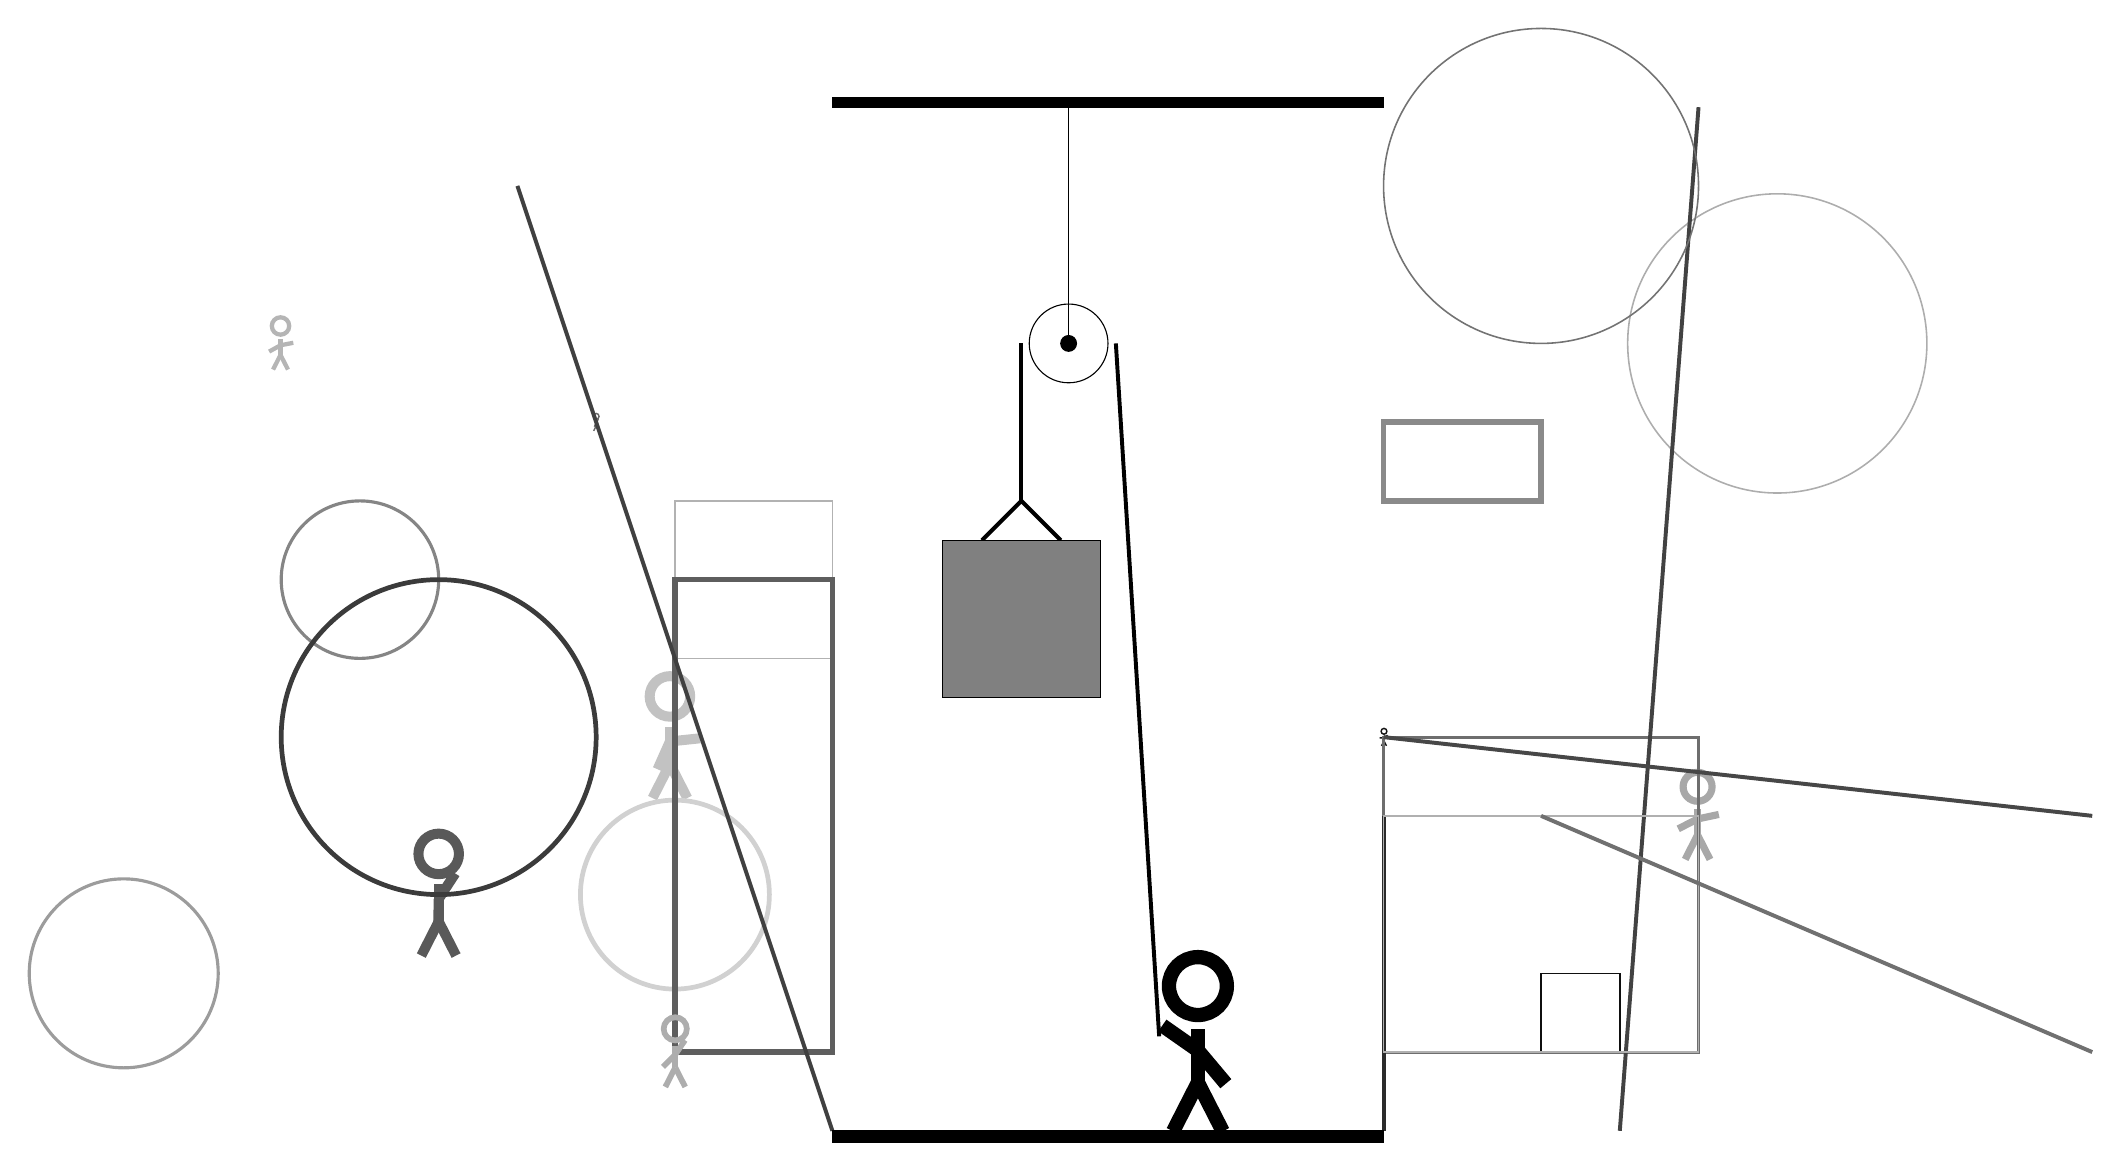
\begin{tikzpicture}
		%%%%% START %%%%%
		
		\draw[fill=black] (-2, 10) rectangle (5, 10.125);
		
		\draw (1, 7) circle (0.5);
		\draw[fill=black] (1, 7) circle (0.1);
		\draw (1, 10) -- (1, 7);
		
		\node[line width=0.4mm, color=black!59] at (-5, 6) {\Strichmaxerl[1][65][59]};
		
		\node[line width=0.7mm, color=black!92] at (5, 2) {\Strichmaxerl[1][2][36]};
		\node[line width=0.5mm, color=black!34] at (9, 1) {\Strichmaxerl[5][27][12]};
		\draw[line width=0.2mm, color=black!30] (-4, 5) rectangle (-2, 3);
		\draw[line width=0.4mm, color=black!57] (5, 2) rectangle (9, -2);
		
		\draw [line width=0.2mm, color=black!32](10, 7) circle (1.9);
		
		\draw [line width=0.4mm, color=black!48](-8, 4) circle (1.0);
		\node[line width=0.6mm, color=black!24] at (-4, 2) {\Strichmaxerl[7][66][6]};
		\draw[line width=0.5mm, color=black!74](9, 10) -- (8, -3);
		\draw[line width=0.5mm, color=black!72](5, 2) -- (14, 1);
		\draw[line width=0.2mm, color=black!94] (7, -2) rectangle (8, -1);
		\draw[line width=0.5mm, color=black!83](5, 1) -- (5, -3);
		\node[line width=0.2mm, color=black!65] at (-7, 0) {\Strichmaxerl[7][89][57]};
		
		\draw [line width=0.2mm, color=black!55](7, 9) circle (2.0);
		\draw [line width=0.6mm, color=black!18](-4, 0) circle (1.2);
		\draw [line width=0.6mm, color=black!77](-7, 2) circle (2.0);
		
		\node[line width=0.6mm, color=black!29] at (-9, 7) {\Strichmaxerl[3][29][11]};
		\draw[line width=0.2mm, color=black!31] (5, 1) rectangle (9, -2);
		\draw[line width=0.7mm, color=black!63] (-2, -2) rectangle (-4, 4);
		\draw[line width=0.5mm, color=black!75](-6, 9) -- (-2, -3);
		\draw[line width=0.5mm, color=black!56](7, 1) -- (14, -2);
		\draw[line width=0.7mm, color=black!46] (7, 5) rectangle (5, 6);
		\node[line width=0.5mm, color=black!32] at (-4, -2) {\Strichmaxerl[4][45][56]};
		\draw [line width=0.4mm, color=black!39](-11, -1) circle (1.2);
		
		\draw[line width=0.5mm] (-0.1, 4.5) -- (0.4, 5.0) -- (0.9, 4.5);
		\draw[fill=black!50] (-0.6, 4.5) rectangle (1.4, 2.5);
		
		\draw[line width=0.5mm] (0.4, 7) -- (0.4, 5.0);
		\centerarc[line width=0.5mm](1, 7)(0:180:0.6);
		\draw[line width=0.5mm](1.6, 7) -- (2.15, -1.8);
		
		\node at (2.6, -1.9) {\Strichmaxerl[10][-35][-50]};
		
		\draw[fill=black] (-2, -3) rectangle (5, -3.15);
		
		%%%%% END %%%%%
	\end{tikzpicture}
\end{document}